
% la.tex
\documentclass[UTF8,a5paper,12pt,portrait,openary,final]{ctexbook}
\usepackage[colorlinks=true,
            linkcolor=black
            ]{hyperref}                               %目錄跳轉
% documentclass not change page size, this one does
\usepackage[b5paper,text={125mm,195mm},centering]{geometry}
%\usepakage{graphics}
%\usepakage{graphicx}

%\usepackage{makeidx}     % -- for 檢索 --
%\makeindex %  生成检索
%\setlength{\baselineskip}{24pt}  % 修改行距
%在编译时,先用 xelatex/pdflatex 编译,接着用 makeindex 编译,最后再
%用 xelatex/pdflatex 编译,才能得到带全文索引的文档。


\usepackage{amscd}      % 画交换图
\usepackage[all]{xy}     % 画交换图的另一个包




\begin{document}


\title{Notes On LaTeX Typesetting}
\author{Some One}
\date{November 13, 2011}
\maketitle


\ctexset{
abstractname = {本文概要},
bibname = {文\quad 献}
}

\tableofcontents    % 目录
%\listoffigures      % 插图目录
%\listoftables       % 表格目录


\clearpage
\addcontentsline{toc}{chapter}{\indexname}
\addcontentsline{toc}{section}{章节描述}
\addcontentsline{lof}{figure}{插图描述}
\addcontentsline{lot}{table}{表格描述}
\addcontentsline{toc}{chapter}{\bibname}

\printindex
\newpage


\xymatrix{
M \ar[rr]^{f}\ar[dr]_{h} &   & N \ar@{-->}[dl]^{g}\\
& P &
}

\xymatrix{
M &   & N \\
& P &
}

\[
\[
\begin{CD}
DT @>f_1>> BJ \\
@Vf_2VV @AAg_1A  \\
HZ @<<g_2< HD
\end{CD}
\]
\]

\[
\[
\begin{CD}
A @>f_1>> B \\
@Vf_2VV @AAg_1A  \\
C @<<g_2< D
\end{CD}
\]
\]









\setlength{\baselineskip}{12pt plus 2pt minus 1pt}

在在T E X中,默认的行距通常是字体大小的1.2倍。如果字体大小为10pt,默认行距 baselineskip将为12pt
。若要调整行距,可以直接修改 baselineskip
的值。例如下面命令将调整行距为双倍行距:

\setlength{\baselineskip}{4pt}
其中,在L A T E X中\setlength命令用于修改各种长度的值。T E X中,默认的行距通常是字体大小的1.2倍。如果字体大小为10pt,默认行距baselineskip将为12pt。若要调整行距,可以直接修改
baselineskip的值。例如下面命令将调整行距为双倍行距
命令用于修改各种长度的值。
命令用于修改各种长度的值。命令用于修改各种长度的值。命令用于修改各种长度的值。

{\linespread{4}\selectfont 命令用于修改各种长度的值。
其中,在L A T E X中setlength
命令用于修改各种长度的值。
}

\linespread{1}\selectfont

\begin{figure}[htbp!]
\centering
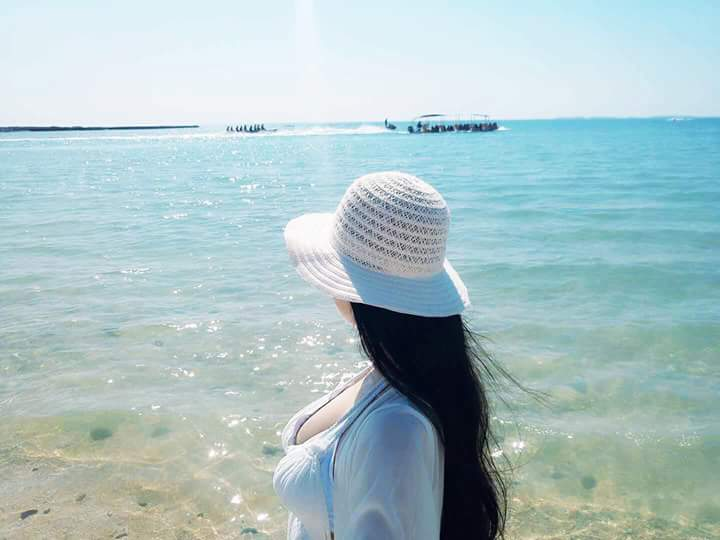
\includegraphics[scale=0.3]{picture/sea.jpg}
\caption{浮动图片自动调整位置}
\label{fig:float}
\end{figure}


\\


\renewcommand\arraystretch{1.5}     % 调整表格行距
\begin{table}[htbp!]
\centering
\begin{tabular}{|l|c|r|l|}
\hline
第一行&第一行&第一行&第一行\\
\hline
第二行&第二行&第二行&第二行\\
\hline
第一行&第一行&第一行&第一行\\
\hline
第二行&第二行&第二行&第二行\\
\hline
\end{tabular}
\caption{浮动表格例子}
\label{tab:float}
\end{table}

\\ 
\begin{table}[htbp!]
\centering
\begin{tabular}{|c|c|c|}
\hline
第一行&第一行&第一行\\
\hline
\multicolumn{2}{|c|}{跨列} &第二行\\
\hline
第三行&第三行&第三行\\
\hline
第四行 & \multicolumn{2}{|c|}{跨列}\\
\hline
\end{tabular}
\caption{浮动表格例子}
\label{tab:float}
\end{table}



\\
\begin{table}[htbp!]
\centering
\begin{tabular}{|l|c|r|}
\hline
左列&中列&右列\\
\hline
第二行&第二行&第二行\\
\hline
左三&中三&右三\\
\hline
\end{tabular}
\caption{浮动表格例子}
\label{tab:float}
\end{table}





正常在黄昏融化了世界的色彩以前正常在黄
\raisebox{-2mm}{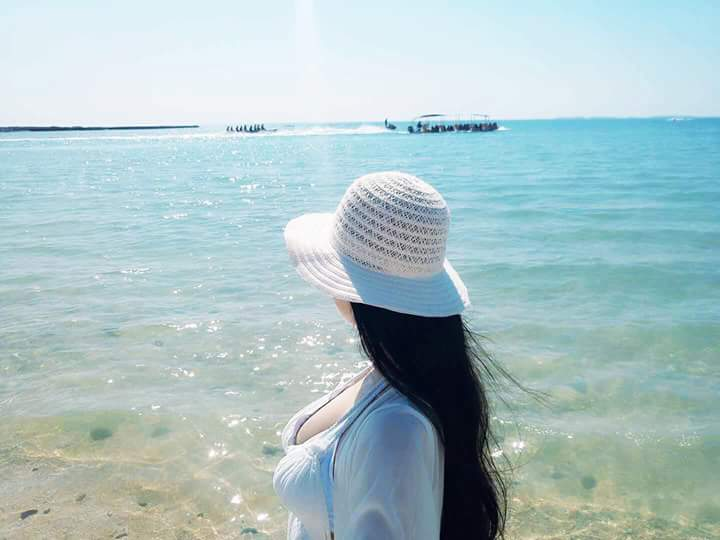
\includegraphics[scale=0.03]{picture/sea.jpg}}
昏融化了世界的色彩以前正常在黄昏融化了世界的色彩以前正常在黄昏融化了世界的色彩以前
正常中国人民解放军\rotatebox{25}{逆时针}正常在黄昏融化了世界的色彩以前
正常在黄昏融化了世界的色彩以前正常在黄昏融化了世界的色彩以前正常在黄昏融化了世界的色彩以前正常在黄昏融化了世界的色彩以前
正常中国人民解放军\rotatebox{25}{逆时针}正常在黄昏融化了世界的色彩以前
正常在黄昏融化了世界的色彩以前正常在黄昏融化了世界的色彩以前正常在黄昏融化了世界的色彩以前正常在黄昏融化了世界的色彩以前
\\
正常\rotatebox{-30}{顺时针}正常
\\
正常\scalebox{-1}[1]{翻转}正常
\\
正常\reflectbox{翻转}正常
\\

正常\scalebox{-1.6}[0.7]{矮胖}正常
\\
正常\scalebox{0.7}[-1.6]{瘦高}正常
\\



正常\scalebox{1.6}[0.7]{矮胖}正常
\\
正常\scalebox{0.7}[1.6]{瘦高}正常
\\
正常\scalebox{1.6}{胖高}正常

\\

正常\resizebox{30pt}{5pt}{矮胖}正常
\\正常\resizebox{11pt}{13pt}{瘦高}正常
\\正常\resizebox{30pt}{!}{胖高}正常




\\
中华\\
人民{\huge 共和国}\\
解放军\smash{军部} 关门

\\







\chapter{章标题}
这一章我们介绍这些内容。
\section{节标题}
这一节我们介绍这些内容。
\subsection{小节标题}
这一小节我们介绍这些内容。
\subsubsection{子节标题}
这一子节我们介绍这些内容。
\paragraph{段标题}
这一段我们介绍这些内容。

D. Knuth wrote some books, e.g. \cite{DK1, DK2}.
\subparagraph{小段标题}
这一小段我们介绍这些内容。







\\
正文正文正文\\
正文\raisebox{6pt}[30pt][3pt]{\fbox{上升}}正文


\\


他的师父是\raisebox{10pt}{\huge 上}真\raisebox{3pt}{\fbox{下}}华
\\
正文\raisebox{-6pt}{\fbox{下降}}正 {\tiny 文}

\\



正文正文
\\
正文\hphantom{水平幻影}正文
\\
正文\vphantom{\Huge竖直幻影}正文



\fbox{a} \fbox{A} \quad
\fbox{a\rule{0pt}{7pt}}
\fbox{A\rule{0pt}{7pt}}
默认\rule{3pt}{14pt}默认
上升\rule[5pt]{3pt}{14pt}上升
下降\rule[-5pt]{3pt}{14pt}下降
\\


正文\mbox{盒子}正文\fbox{盒子}正文

正文
\makebox[10em][r]{靠右对齐}正文\\
正文\framebox[10em][r]{靠右对齐}正文

Left\begin{minipage}{6em}
One\\ Two\\ Three
\end{minipage}Right

\begin{abstract}
some abstract
\end{abstract}


Left\parbox{6em}{One\\ Two\\ Three}Right

\\
Left\fbox{\begin{minipage}{6em}
One\\ Two\\ Three
\end{minipage}}Right


\newtheorem{aaa}{Theorem}
\newtheorem{bbb}{Corollary}

\begin{aaa}
This is a theorem.
\end{aaa}
\begin{bbb}
This is a corollary.
\end{bbb}

\begin{thebibliography}{123456}
\bibitem[mag]{DK1} D. Li, T.A.O.C.P. , Vol. 1, Addison-Wesley, 1997.
\bibitem[ray]{DK2} D. Jiang, T.A.O.C.P. , Vol. 2, Addison-Wesley, 1999.
\bibitem[Knuth3]{DK3} D. Knuth, T.A.O.C.P. , Vol. 3, Addison-Wesley, 1998.
\end{thebibliography}

\end{document}

